\section{Evaluation Setup}

\begin{frame}
  \sectionpage
\end{frame}



% \begin{frame}{Introduction to Poisoning Attacks}
%   \begin{itemize}
%     \item By \emph{component}:
%     \begin{itemize}
%       \item Data poisoning (\eg, \alert<5>{label-flipping}, clean-label attacks, backdoors)
%       \item Model poisoning (\eg, gradient boosting, noising)
%     \end{itemize}\emph{}

%     \pause
%     \item By \emph{target}:
%     \begin{itemize}
%       \item \alert<5>{Untargeted}: affect the model's global performance
%       \item \alert<5>{Targeted}: modify its behavior on specific classes or instances
%     \end{itemize}

%     \pause
%     \item By \emph{frequency}:
%     \begin{itemize}
%       \item one-shot: attacks are performed once
%       \item \alert<5>{iterative}/\alert<5>{continuous}: at each round
%       \item adaptive: reacts to the model aggregation
%     \end{itemize}

%     \pause
%     \item By \emph{proportion}:
%     \begin{itemize}
%       \item \alert<5>{Lone}: single attacker.
%       \item \alert<5>{Colluding minority}: several colluding attackers, outnumbered by benign participants. 
%       \item \alert<5>{Colluding majority}: several colluding attackers outnumbering benign participants.
%     \end{itemize}
%   \end{itemize}
% \end{frame}

\newtcolorbox{taxobox}[1][]{
  enhanced,
  colback=imta-blue!5,
  colbacktitle=imta-blue,
  coltitle=white,
  sharp corners,
  frame hidden,
  boxrule=0pt,
  fontupper=\small,
  fonttitle=\bfseries,
  after title app=\strut,
  height=3cm,
  title=#1
}


\begin{frame}{Introduction to Poisoning Attacks}
  \vspace{1em}
  
  \setlength{\leftmargini}{5pt}
  \begin{tcbraster}[raster columns=2, raster equal height, raster column skip=2em, raster row skip=2em]
    \pause
    \begin{taxobox}[By \emph{component}]
      \begin{itemize}
        \item Data poisoning (\eg, \textbf<5>{label-flipping}, clean-label)
        \item Model poisoning (\eg, gradient boosting)
      \end{itemize}
    \end{taxobox}
    \pause
    \begin{taxobox}[By \emph{objective}]
      \begin{itemize}
        \item Untargeted: impact model performance
        \item Targeted: modify behavior for specific samples
      \end{itemize}
    \end{taxobox}
    \pause
    \begin{taxobox}[By \emph{timing}]
      \begin{itemize}
        \item one-shot: performed once
        \item \textbf<5>{incremental/continuous}: at each round
      \end{itemize}
    \end{taxobox}
    \pause
    \begin{taxobox}[By \emph{proportion}]
      \begin{itemize}
        \item Single attacker
        \item Colluding attackers: multiple coordinated participants
      \end{itemize}
    \end{taxobox}
  \end{tcbraster}
\end{frame}



\begin{frame}{Simulating Practical Heterogeneity}
% Repère oral : dire que c'est 1/5 des données par participants de manières exclusive. 
  \begin{columns}
    \begin{column}{.5\textwidth}
      \textbf{Datasets}
      \begin{itemize}
        \item Heterogeneous datasets, but some participants can share similarities.
        \item 4 datasets: CIC-CSE-IDS2018, UNSW-NB15, Bot-IoT, ToN\_IoT.
        \item NF-V2~\autocite{sarhan_StandardFeatureSet_2021} feature set (\ie, NetFlow V9).
      \end{itemize}
    \end{column}
    \begin{column}{.5\textwidth}
      \begin{figure}
        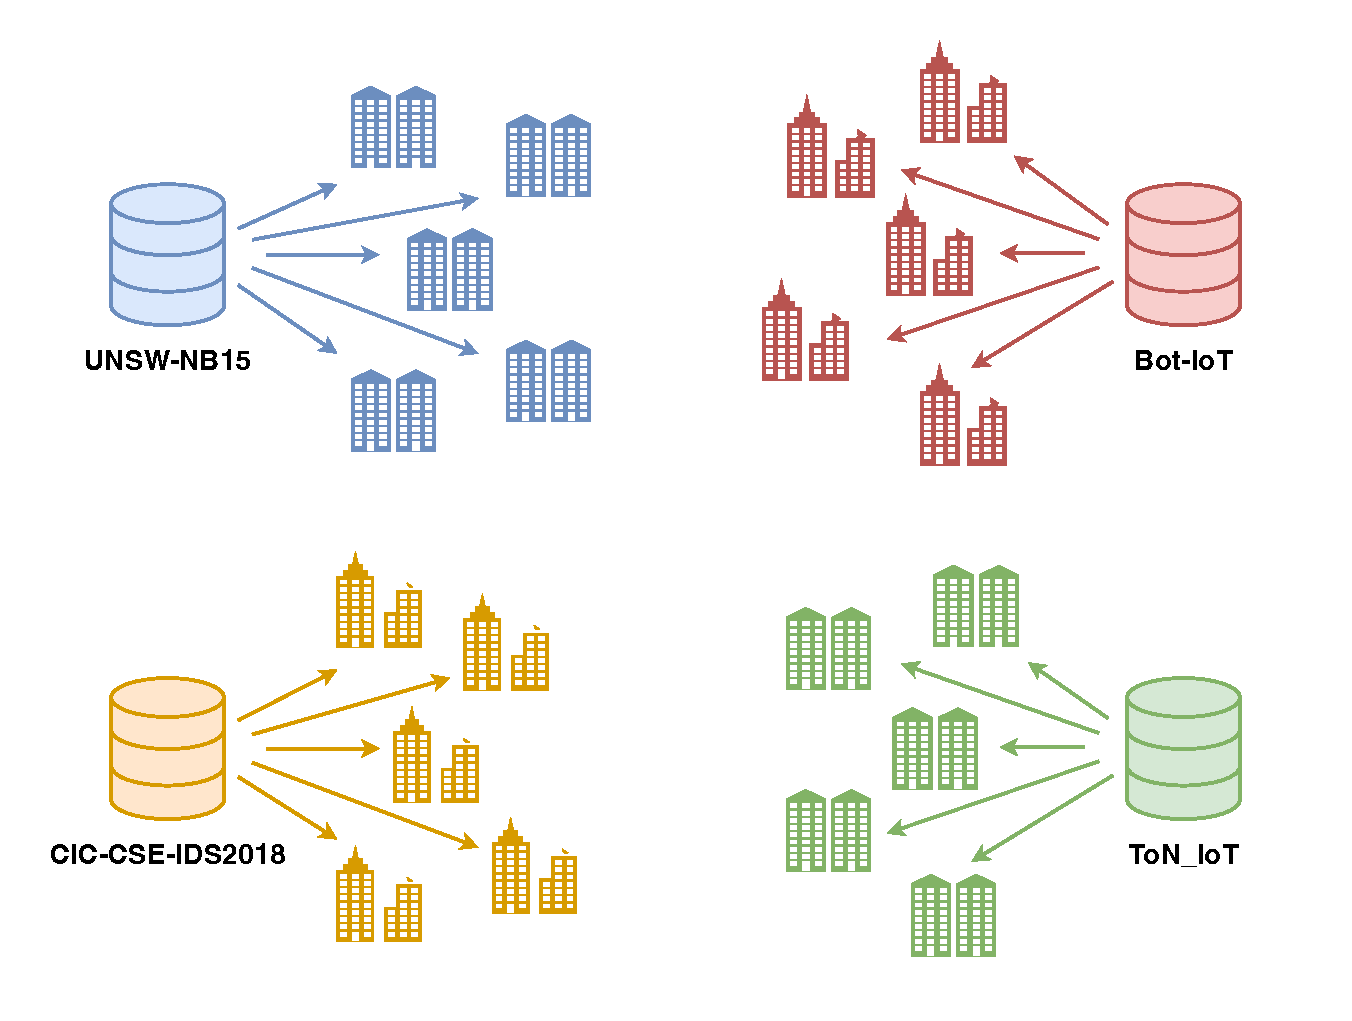
\includegraphics[width=\linewidth]{figures/eval/setup/partition.pdf}%
      \end{figure}
    \end{column}
  \end{columns}
  \fcitefootnote{sarhan_StandardFeatureSet_2021}
\end{frame}

\begin{frame}{Attack scenarios}
    \begin{columns}
        \begin{column}{.5\textwidth}
            \textbf{Parameters}
            \begin{itemize}
                \item \textit{Target}: Affected classes.
                \item \textit{Data Poisoning Rate (DPR)}: proportion of targeted data with flipped labels.
                \item \textit{Model Poisoning Rate (MPR)}: number of attackers in the cluster.
            \end{itemize}
        \end{column}
        \begin{column}{.5\textwidth}
          \begin{figure}
            \captionsetup{font=small, labelfont=small}
            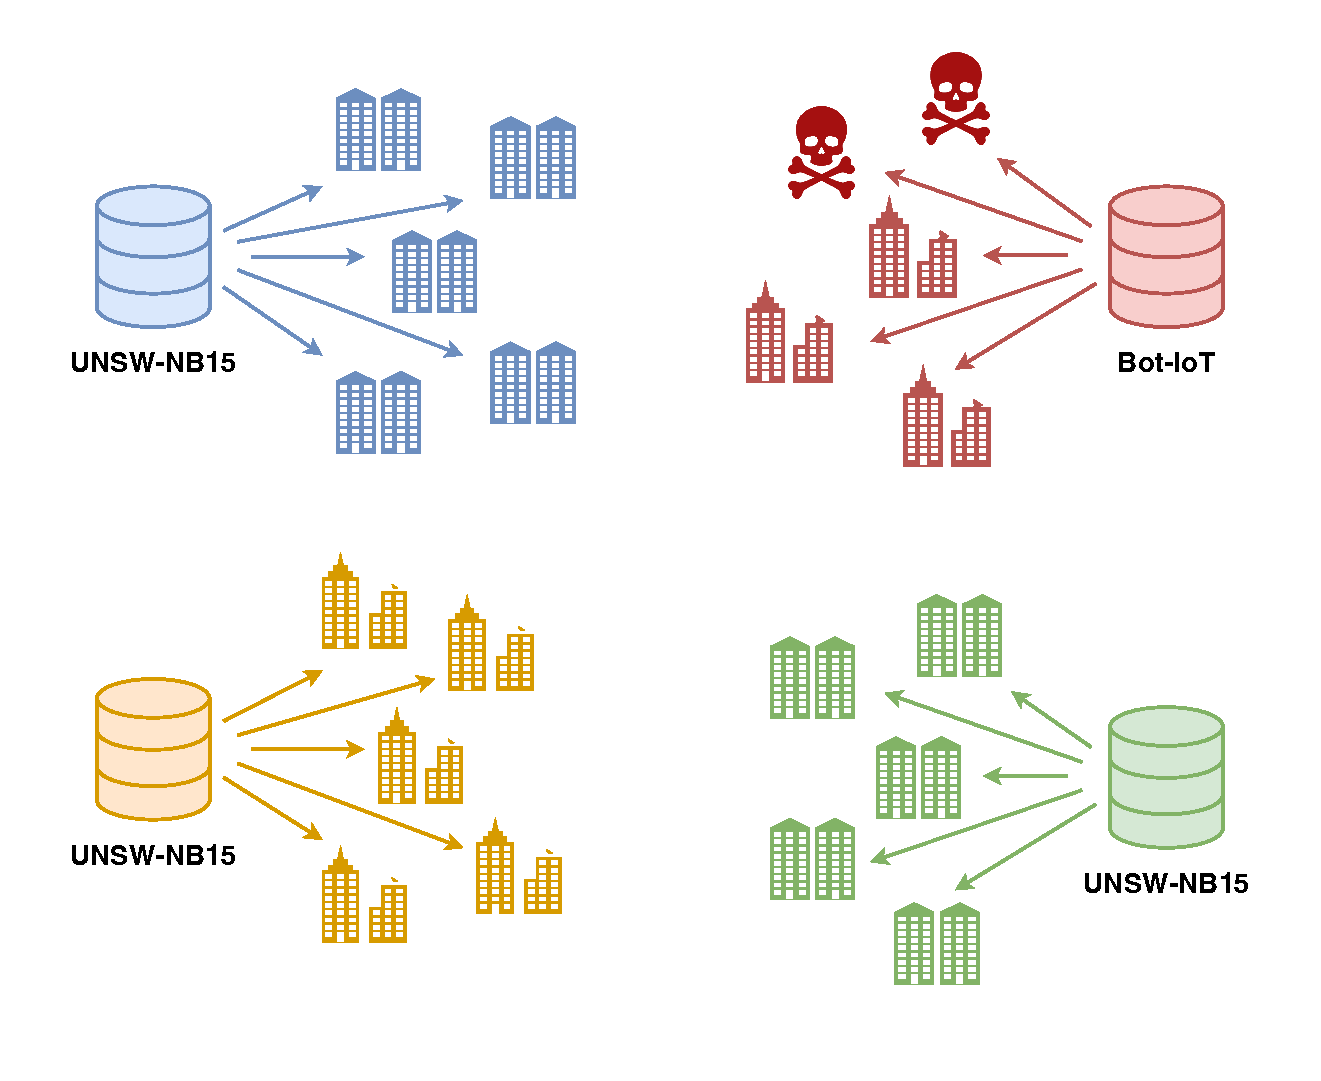
\includegraphics[width=\linewidth]{figures/eval/setup/poisoning.pdf}%
            \caption{\texttt{colluding minority 100T} (\ie, 2 attackers, 100\% data poisoning on Reconnaissance class).}
          \end{figure}
        \end{column}
    \end{columns}
\end{frame}

% \begin{frame}{Experimental Setup: attack scenarios}
%   \begin{columns}
%     \begin{column}{.55\textwidth}
%       \texttt{colluding majority 100U:}
%       \begin{itemize}
%         \item \texttt{colluding majority}: \alert{3} out of 5 participants from Bot-IoT are attackers.
%         \item \texttt{100}: 100\% of their datas are flipped.
%         \item \texttt{U}: on \alert{all} attack classes. 
%         \end{itemize}
%     \end{column}
%     \begin{column}{.45\textwidth}
%       \begin{figure}
%         \centering
%         \captionsetup{justification=centering}
%         \caption{Participants for \texttt{colluding majority 100U}.}
%       \end{figure}
%     \end{column}
%   \end{columns}
% \end{frame}

% \begin{frame}{Experimental Setup: attack scenarios}
%   \begin{columns}
%     \begin{column}{.55\textwidth}
%       \texttt{colluding minority 100T:}
%       \begin{itemize}
%         \item \texttt{colluding minority}: \alert{2} out of 5 participants from Bot-IoT are attackers.
%         \item \texttt{100}: 100\% of their data are flipped.
%         \item \texttt{T}: on the \alert{Reconnaissance} class only. 
%         \end{itemize}
%     \end{column}
%     \begin{column}{.45\textwidth}
%       \begin{figure}
%       \centering
%         \captionsetup{justification=centering}
%         \includegraphics<1>[width=.80\linewidth]{figures/eval/setup/min_targeted.pdf}%
%         \caption{Participants for \texttt{colluding minority 100T}.}
%       \end{figure}
%     \end{column}
%   \end{columns}
% \end{frame}


\begin{frame}{Comparison Baselines}
      \begin{itemize}
        \item \texttt{RADAR}: Our framework.
        \item \texttt{FoolsGold}: Similarity-based mitigation strategy in NIID\footnote{Not Independent nor Identically Distributed (NIID)}. settings~\cite{fung_LimitationsFederatedLearning_2020}.
        \item \texttt{FedAvg}: the original FL algorithm~\cite{mcmahan_Communicationefficientlearningdeep_2017}.
        \item \texttt{FedAvg} with \emph{ideal} clustering.
      \end{itemize}
\end{frame}
